% 原书印刷页4–16（至1.3节前）；PDF物理页35–47.逐页核对原图.
\subsection{概率论}\label{sec:1.2}
进行一次试验时，其实现是样本空间中的一个结果.若把试验重复多次，每次可能出现不同的结果，也可能重复出现某些结果.一个结果的这种“出现频率”可以看作一种概率.概率较大的结果出现得更频繁.如果能够用概率来描述试验的结果，我们就迈出了用统计方法分析试验的一步.

本节介绍概率论的一些基础知识.我们不以频率来定义概率，而是采用数学上更简单的公理化方法.正如将要看到的，公理化方法不关心概率的解释，只关心概率是否由满足公理的函数定义.概率的解释是另一回事.事件的“出现频率”就是概率的一种特定解释.另一种可能的解释是主观解释：不把概率看作频率，而把它看作对某事件发生机会的信念.


\sourcepageanchor{36}

\subsubsection{公理化基础}\label{sec:1.2.1}
对样本空间$S$中的每个事件$A$，我们希望给它赋予一个介于0和1之间的数，称为$A$的概率，记作$P(A)$.似乎很自然，可以把$P$的定义域（函数$P(\cdot)$的自变量所在的集合）定义为$S$的所有子集；也就是说，对每个$A\subset S$，定义$P(A)$为$A$发生的概率.不幸的是，事情没有这么简单.有一些技术困难需要克服.我们不详谈这些技术细节；虽然它们很重要，但概率论学家通常比统计学家更关心它们.不过，要扎实地理解统计学，至少应对以下内容略知一二.
\begin{definition}\label{def:1.2.1}\index{SI0097@博雷尔域（见$\sigma$代数）}\index{SI0972@$\sigma$代数}
$S$的一个子集族若满足以下三个性质，就称为一个\emph{$\sigma$代数}（sigma algebra，或Borel field），记作$\mathscr B$：
\begin{enumerate}
\item[(a)]\phantomsection\label{itm:def:1.2.1:a} $\emptyset\in\mathscr B$（空集是$\mathscr B$的一个元素）.
\item[(b)]\phantomsection\label{itm:def:1.2.1:b} 若$A\in\mathscr B$，则$A^c\in\mathscr B$（$\mathscr B$对取补运算封闭）.
\item[(c)] 若$A_1,A_2,\ldots\in\mathscr B$，则$\bigcup_{i=1}^{\infty}A_i\in\mathscr B$（$\mathscr B$对可数并封闭）.
\end{enumerate}
\end{definition}
空集$\emptyset$是任何集合的子集，因此$\emptyset\subset S$.性质\hyperref[itm:def:1.2.1:a]{(a)}说明，这个子集总属于一个$\sigma$代数.因为$S=\emptyset^c$，性质\hyperref[itm:def:1.2.1:a]{(a)}与\hyperref[itm:def:1.2.1:b]{(b)}还说明$S$总属于$\mathscr B$.此外，由德摩根律可知\index{SI0247@德摩根律（见集合运算）}\semanticindexanchor{247:36}，$\mathscr B$对可数交也封闭.若$A_1,A_2,\ldots\in\mathscr B$，则由性质\hyperref[itm:def:1.2.1:b]{(b)}有$A_1^c,A_2^c,\ldots\in\mathscr B$，因此$\bigcup_{i=1}^{\infty}A_i^c\in\mathscr B$.不过，利用德摩根律（如习题\ref{exercise:1.9}所示），有
\begin{equation}\label{eq:1.2.1}
\left(\bigcup_{i=1}^{\infty}A_i^c\right)^c=\bigcap_{i=1}^{\infty}A_i.
\end{equation}
因此，再用性质\hyperref[itm:def:1.2.1:b]{(b)}，得$\bigcap_{i=1}^{\infty}A_i\in\mathscr B$.

与样本空间$S$相联系的$\sigma$代数可以有许多个.例如，由两个集合组成的集合族$\{\emptyset,S\}$就是一个$\sigma$代数，通常称为平凡$\sigma$代数.\index{SI0976@平凡}\semanticindexanchor{976:36}我们只关心包含给定样本空间$S$中所有开集的最小$\sigma$代数.
\begin{example}[$\sigma$代数——I]\label{ex:1.2.2}\index{SI0973@可数}
若$S$有限或可数，这些技术困难其实不会出现，因为对给定样本空间$S$，我们定义
$$\mathscr B=\{S\text{ 的所有子集，包括 }S\text{ 本身}\}.$$
若$S$有$n$个元素，则$\mathscr B$中有$2^n$个集合（见习题\ref{exercise:1.14}）.例如，若$S=\{1,2,3\}$，则$\mathscr B$是以下$2^3=8$个集合组成的集合族：
$$\begin{array}{ccc}
\{1\}&\{1,2\}&\{1,2,3\}\\[3pt]
\{2\}&\{1,3\}&\emptyset\\[3pt]
\{3\}&\{2,3\}&
\end{array}$$
\end{example}
一般说来，若$S$不可数，描述$\mathscr B$并不容易.不过，我们选取的$\mathscr B$会包含所有感兴趣的集合.
\begin{example}[$\sigma$代数——II]\label{ex:1.2.3}\index{SI0977@不可数}
令$S=(-\infty,\infty)$为实数轴.选取$\mathscr B$使其包含对所有实数$a,b$所形成的下列各类集合：
$$[a,b],\quad(a,b],\quad(a,b),\quad\text{和}\quad[a,b).$$
此外，由$\mathscr B$的性质可知，它还包含对上述各类集合取并和交（可能为可数无穷次）所能得到的一切集合.
\end{example}
现在可以定义概率函数了.

\sourcepageanchor{37}

\begin{definition}\label{def:1.2.4}\index{SI0596@柯尔莫哥洛夫公理}\index{SI0843@概率函数}
给定样本空间$S$及与之相联系的$\sigma$代数$\mathscr B$，\emph{概率函数}（probability function）是以$\mathscr B$为定义域、满足下列条件的函数$P$：
\begin{enumerate}[label=\arabic*.]
\item 对所有$A\in\mathscr B$，$P(A)\ge0$.
\item $P(S)=1$.
\item 若$A_1,A_2,\ldots\in\mathscr B$两两不相交，则$P(\bigcup_{i=1}^{\infty}A_i)=\sum_{i=1}^{\infty}P(A_i)$.
\end{enumerate}
\end{definition}
定义\ref{def:1.2.4}中的三个性质通常称为概率公理（Axioms of Probability），或柯尔莫哥洛夫公理（Kolmogorov Axioms），以概率论奠基人之一A. Kolmogorov命名.满足概率公理的任何函数$P$都称为概率函数.公理化定义不打算告诉我们应该选择哪个具体的函数$P$；它只要求$P$满足这些公理.对任意样本空间，都可以定义许多不同的概率函数.哪些函数能够反映某一特定试验中可能观察到的情形，还有待讨论.
\begin{example}[定义概率——I]\label{ex:1.2.5}
考虑抛一枚公平硬币的简单试验，此时$S=\{\mathrm H,\mathrm T\}$.所谓“公平”，是指硬币平衡，正面朝上和反面朝上的可能性相同.因此，合理的概率函数应赋予正面和反面相等的概率，即
\begin{equation}\label{eq:1.2.2}
P(\{\mathrm H\})=P(\{\mathrm T\}).
\end{equation}
注意，式\eqref{eq:1.2.2}并非概率公理的推论，而是公理之外的要求.我们使用了概率的对称性解释（或者仅凭直觉），要求正面与反面等可能.因为$S=\{\mathrm H\}\cup\{\mathrm T\}$，由公理2得$P(\{\mathrm H\}\cup\{\mathrm T\})=1$.又因为$\{\mathrm H\}$和$\{\mathrm T\}$不相交，$P(\{\mathrm H\}\cup\{\mathrm T\})=P(\{\mathrm H\})+P(\{\mathrm T\})$，于是
\begin{equation}\label{eq:1.2.3}
P(\{\mathrm H\})+P(\{\mathrm T\})=1.
\end{equation}
联立式\eqref{eq:1.2.2}和\eqref{eq:1.2.3}，得$P(\{\mathrm H\})=P(\{\mathrm T\})=\frac12$.

由于式\eqref{eq:1.2.2}依据的是我们对具体试验的了解，而不是公理，因此，只要$P(\{\mathrm H\})$和$P(\{\mathrm T\})$取非负值并满足式\eqref{eq:1.2.3}，就定义了一个合法的概率函数.例如，可以取$P(\{\mathrm H\})=\frac19$和$P(\{\mathrm T\})=\frac89$.
\end{example}
我们需要一些定义概率函数的一般方法，并且知道它们总能满足柯尔莫哥洛夫公理.我们不希望每引入一个新的概率函数，都像例\ref{ex:1.2.5}那样逐一检查公理.下面给出一种定义合法概率函数的常用方法.
\begin{theorem}\label{thm:1.2.6}\index{SI0844@有限集}
设$S=\{s_1,\ldots,s_n\}$是有限集，$\mathscr B$是$S$的子集构成的任意$\sigma$代数，$p_1,\ldots,p_n$是和为1的非负数.对任意$A\in\mathscr B$，定义
$$P(A)=\sum_{\{i:s_i\in A\}}p_i.$$
（空集上的求和定义为0.）则$P$是$\mathscr B$上的概率函数.若$S=\{s_1,s_2,\ldots\}$为可数集，结论仍然成立.
\end{theorem}
\begin{proof}
我们证明$S$有限的情形.对任意$A\in\mathscr B$，$P(A)=\sum_{\{i:s_i\in A\}}p_i\ge0$，因为每个$p_i\ge0$.所以公理1成立.
$$P(S)=\sum_{\{i:s_i\in S\}}p_i=\sum_{i=1}^n p_i=1.$$
所以公理2成立.令$A_1,\ldots,A_k$表示两两不相交的事件.（$\mathscr B$只含有限个集合，因此只需考虑有限个互不相交集合的并.）于是，
$$P\left(\bigcup_{i=1}^k A_i\right)=\sum_{\{j:s_j\in\bigcup_{i=1}^k A_i\}}p_j
=\sum_{i=1}^k\sum_{\{j:s_j\in A_i\}}p_j=\sum_{i=1}^k P(A_i).$$
第一个和第三个等号来自$P(A)$的定义.$A_i$互不相交保证了第二个等号，因为等号两边相同的$p_j$各出现恰好一次.因此公理3成立，柯尔莫哥洛夫公理全部满足.
\end{proof}
试验的物理实际可能决定概率如何分配，下面的例子说明了这一点.

\sourcepageanchor{38}

\begin{figure}[htbp]\centering
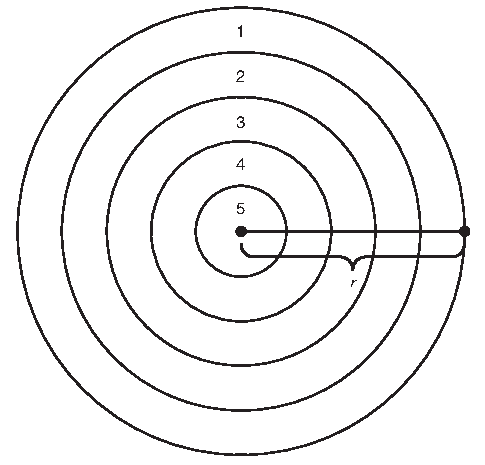
\includegraphics[width=.52\textwidth]{assets/chapter1/fig1-2-1.pdf}
\caption{例\ref{ex:1.2.7}中的飞镖靶}\label{fig:1.2.1}
\end{figure}
\begin{example}[定义概率——II]\label{ex:1.2.7}
飞镖游戏中，选手向靶上投掷飞镖，所得分数等于飞镖落入区域所标的数.对初学者而言，假设飞镖命中某个区域的概率与该区域面积成正比，似乎是合理的.因此，面积较大的区域被命中的概率较高.

如图\ref{fig:1.2.1}所示，飞镖靶的半径为$r$，相邻圆环之间的距离为$r/5$.若假设总能命中靶面（习题\ref{exercise:1.7}给出一个变式），则
$$P(\text{得到 }i\text{ 分})=\frac{\text{区域 }i\text{ 的面积}}{\text{飞镖靶面积}}.$$
例如，
$$P(\text{得到1分})=\frac{\pi r^2-\pi(4r/5)^2}{\pi r^2}=1-\left(\frac45\right)^2.$$
一般公式很容易导出，结果为
$$P(\text{得到 }i\text{ 分})=\frac{(6-i)^2-(5-i)^2}{5^2},\qquad i=1,\ldots,5,$$
与$\pi$和$r$无关.各个互不相交区域的面积之和等于靶面积.因此赋予这五个结果的概率之和为1，由定理\ref{thm:1.2.6}可知，这确实是一个概率函数（习题\ref{exercise:1.8}）.
\end{example}
在结束概率的公理化讨论之前，还有一点需要考虑.定义\ref{def:1.2.4}中的公理3，通常称为可数可加性公理（Axiom of Countable Additivity）\index{SI0074@可数可加性公理}\semanticindexanchor{74:38}，并未得到所有统计学家的认可.的确，人们可以认为公理应是简单且不言自明的陈述.与其他简单且不言自明的公理相比，公理3可能使我们怀疑：假定它为真是否合理？

以\hyperref[bib:source95]{De Finetti（1972）}为代表的一个统计学派拒绝可数可加性公理，选择以有限可加性公理取代它.

\noindent\emph{有限可加性公理（Axiom of Finite Additivity）：}\index{SI0075@有限可加性公理}\semanticindexanchor{75:39}若$A\in\mathscr B$与$B\in\mathscr B$不相交，则
$$P(A\cup B)=P(A)+P(B).$$
虽然这个公理未必完全不言自明，但它当然比可数可加性公理简单（并且可由后者推出，见习题\ref{exercise:1.12}）.

只假定有限可加性也许更可信，但会在统计理论中导致意想不到的复杂情况；在本书的层次上，这些复杂情况不一定有助于理解.因此，以下均假定可数可加性公理成立.

\subsubsection{概率的运算}\label{sec:1.2.2}
从概率公理出发，可以建立概率函数的许多性质，它们对计算较复杂的概率很有帮助.本节详细讨论其中一些运算，另一些留作习题.

先从概率函数应用于单个事件时的一些（相当明显的）性质开始.

\sourcepageanchor{39}

\begin{theorem}\label{thm:1.2.8}\index{SI0846@性质}
若$P$是概率函数，$A$是$\mathscr B$中的任意集合，则
\begin{enumerate}
\item[(a)]\phantomsection\label{itm:thm:1.2.8:a} $P(\emptyset)=0$，其中$\emptyset$是空集；
\item[(b)]\phantomsection\label{itm:thm:1.2.8:b} $P(A)\le1$；
\item[(c)]\phantomsection\label{itm:thm:1.2.8:c} $P(A^c)=1-P(A)$.
\end{enumerate}
\end{theorem}
\begin{proof}
先证明\hyperref[itm:thm:1.2.8:c]{(c)}最容易.集合$A$与$A^c$构成样本空间的一个划分，即$S=A\cup A^c$.因此，由第二条公理，
\begin{equation}\label{eq:1.2.4}P(A\cup A^c)=P(S)=1.\end{equation}
又因为$A$与$A^c$不相交，由第三条公理，
\begin{equation}\label{eq:1.2.5}P(A\cup A^c)=P(A)+P(A^c).\end{equation}
合并式\eqref{eq:1.2.4}和\eqref{eq:1.2.5}即得\hyperref[itm:thm:1.2.8:c]{(c)}.

因为$P(A^c)\ge0$，\hyperref[itm:thm:1.2.8:c]{(c)}立即推出\hyperref[itm:thm:1.2.8:b]{(b)}.为证明\hyperref[itm:thm:1.2.8:a]{(a)}，对$S=S\cup\emptyset$作类似论证.（回想$S$与$\emptyset$总在$\mathscr B$中.）由于$S$与$\emptyset$不相交，有
$$1=P(S)=P(S\cup\emptyset)=P(S)+P(\emptyset),$$
因此$P(\emptyset)=0$.
\end{proof}
定理\ref{thm:1.2.8}中的性质非常基本，几乎也带有公理的意味，尽管我们已仅用最初的三条柯尔莫哥洛夫公理严格证明了它们.下面的定理与定理\ref{thm:1.2.8}精神相似，但其结论并不那么显然.
\begin{theorem}\label{thm:1.2.9}
若$P$是概率函数，$A$和$B$是$\mathscr B$中的任意集合，则
\begin{enumerate}
\item[(a)]\phantomsection\label{itm:thm:1.2.9:a} $P(B\cap A^c)=P(B)-P(A\cap B)$；
\item[(b)]\phantomsection\label{itm:thm:1.2.9:b} $P(A\cup B)=P(A)+P(B)-P(A\cap B)$；
\item[(c)]\phantomsection\label{itm:thm:1.2.9:c} 若$A\subset B$，则$P(A)\le P(B)$.
\end{enumerate}
\end{theorem}
\begin{proof}
为证明\hyperref[itm:thm:1.2.9:a]{(a)}，注意对任意集合$A,B$，有
$$B=\{B\cap A\}\cup\{B\cap A^c\},$$
因此
\begin{equation}\label{eq:1.2.6}
P(B)=P(\{B\cap A\}\cup\{B\cap A^c\})=P(B\cap A)+P(B\cap A^c),
\end{equation}
其中最后一个等号来自$B\cap A$与$B\cap A^c$不相交.移项即得\hyperref[itm:thm:1.2.9:a]{(a)}.

为证明\hyperref[itm:thm:1.2.9:b]{(b)}，使用恒等式
\begin{equation}\label{eq:1.2.7}A\cup B=A\cup\{B\cap A^c\}.\end{equation}
维恩图可以说明式\eqref{eq:1.2.7}为何成立，严格证明也不困难（见习题\ref{exercise:1.2}）.利用式\eqref{eq:1.2.7}及$A$与$B\cap A^c$不相交这一事实（因为$A$与$A^c$不相交），由\hyperref[itm:thm:1.2.9:a]{(a)}得到
\begin{equation}\label{eq:1.2.8}
P(A\cup B)=P(A)+P(B\cap A^c)=P(A)+P(B)-P(A\cap B).
\end{equation}
若$A\subset B$，则$A\cap B=A$.所以利用\hyperref[itm:thm:1.2.9:a]{(a)}，有
$$0\le P(B\cap A^c)=P(B)-P(A),$$
从而\hyperref[itm:thm:1.2.9:c]{(c)}成立.
\end{proof}
定理\ref{thm:1.2.9}的\hyperref[itm:thm:1.2.9:b]{(b)}给出了交事件概率的一个有用不等式.由于$P(A\cup B)\le1$，对式\eqref{eq:1.2.8}作简单移项，得
\begin{equation}\label{eq:1.2.9}\index{SI0560@Bonferroni}P(A\cap B)\ge P(A)+P(B)-1.\end{equation}
它是邦费罗尼不等式（Bonferroni's Inequality）的一个特例［\hyperref[bib:source221]{Miller（1981）}是很好的参考文献］.邦费罗尼不等式使我们可以用单个事件的概率来界定同时发生事件（即交事件）的概率.

\sourcepageanchor{40}

\begin{example}[邦费罗尼不等式]\label{ex:1.2.10}
当交事件的概率很难甚至无法计算，但我们仍希望了解该概率的大小时，邦费罗尼不等式尤其有用.设$A,B$是两个事件，各自的概率都是$.95$，则二者同时发生的概率有下界
$$P(A\cap B)\ge P(A)+P(B)-1=.95+.95-1=.90.$$
注意，除非各个事件的概率足够大，否则邦费罗尼界只是一个没有用处（但正确！）的负数.
\end{example}
本小节最后给出一个定理，其中的结论有助于处理集合族.
\begin{theorem}\label{thm:1.2.11}\index{SI0563@Boole}
若$P$是概率函数，则
\begin{enumerate}
\item[(a)]\phantomsection\label{itm:thm:1.2.11:a} 对任意划分$C_1,C_2,\ldots$，有$P(A)=\sum_{i=1}^{\infty}P(A\cap C_i)$；
\item[(b)]\phantomsection\label{itm:thm:1.2.11:b} 对任意集合$A_1,A_2,\ldots$，有$P(\bigcup_{i=1}^{\infty}A_i)\le\sum_{i=1}^{\infty}P(A_i)$.（布尔不等式，Boole's Inequality）
\end{enumerate}
\end{theorem}
\begin{proof}
由于$C_1,C_2,\ldots$构成划分，对所有$i\ne j$有$C_i\cap C_j=\emptyset$，且$S=\bigcup_{i=1}^{\infty}C_i$.于是
$$A=A\cap S=A\cap\left(\bigcup_{i=1}^{\infty}C_i\right)=\bigcup_{i=1}^{\infty}(A\cap C_i),$$

\sourcepageanchor{41}

最后一个等号来自分配律（定理\ref{thm:1.1.4}）.因此
$$P(A)=P\left(\bigcup_{i=1}^{\infty}(A\cap C_i)\right).$$
由于$C_i$互不相交，集合$A\cap C_i$也互不相交，由概率函数的性质，
$$P\left(\bigcup_{i=1}^{\infty}(A\cap C_i)\right)=\sum_{i=1}^{\infty}P(A\cap C_i),$$
故\hyperref[itm:thm:1.2.11:a]{(a)}成立.

为证明\hyperref[itm:thm:1.2.11:b]{(b)}，先构造一族互不相交的集合$A_1^*,A_2^*,\ldots$，使$\bigcup_{i=1}^{\infty}A_i^*=\bigcup_{i=1}^{\infty}A_i$.定义
$$A_1^*=A_1,\qquad A_i^*=A_i\setminus\left(\bigcup_{j=1}^{i-1}A_j\right),\qquad i=2,3,\ldots,$$
其中$A\setminus B$表示$A$中不与$B$相交的部分.用熟悉的符号表示就是$A\setminus B=A\cap B^c$.不难看出$\bigcup_{i=1}^{\infty}A_i^*=\bigcup_{i=1}^{\infty}A_i$，因此
$$P\left(\bigcup_{i=1}^{\infty}A_i\right)=P\left(\bigcup_{i=1}^{\infty}A_i^*\right)=\sum_{i=1}^{\infty}P(A_i^*),$$
最后一个等号成立是因为$A_i^*$互不相交.为说明这一点，写成
$$\begin{aligned}
A_i^*\cap A_k^*
&=\left\{A_i\setminus\left(\bigcup_{j=1}^{i-1}A_j\right)\right\}\cap\left\{A_k\setminus\left(\bigcup_{j=1}^{k-1}A_j\right)\right\}\quad\text{（$A_i^*$的定义）}\\
&=\left\{A_i\cap\left(\bigcup_{j=1}^{i-1}A_j\right)^c\right\}\cap\left\{A_k\cap\left(\bigcup_{j=1}^{k-1}A_j\right)^c\right\}\quad\text{（$\setminus$的定义）}\\
&=\left\{A_i\cap\bigcap_{j=1}^{i-1}A_j^c\right\}\cap\left\{A_k\cap\bigcap_{j=1}^{k-1}A_j^c\right\}.\quad\text{（德摩根律）}
\end{aligned}$$
若$i>k$，上式第一个交中包含集合$A_k^c$，它与$A_k$的交为空集.若$k>i$，论证相同.此外，由构造可知$A_i^*\subset A_i$，所以$P(A_i^*)\le P(A_i)$，于是
$$\sum_{i=1}^{\infty}P(A_i^*)\le\sum_{i=1}^{\infty}P(A_i),$$
故\hyperref[itm:thm:1.2.11:b]{(b)}成立.
\end{proof}
布尔不等式和邦费罗尼不等式之间有相似之处.\index{SI0559@Bonferroni与Boole的相似性}\semanticindexanchor{559:41}事实上，它们本质上是同一回事.我们本来可以用布尔不等式推出式\eqref{eq:1.2.9}.把布尔不等式用于$A^c$，得
$$P\left(\bigcup_{i=1}^n A_i^c\right)\le\sum_{i=1}^n P(A_i^c),$$
再利用$\bigcup A_i^c=(\bigcap A_i)^c$及$P(A_i^c)=1-P(A_i)$，得到
$$1-P\left(\bigcap_{i=1}^n A_i\right)\le n-\sum_{i=1}^n P(A_i).$$

\sourcepageanchor{42}

移项后变为
\begin{equation}\label{eq:1.2.10}\index{SI0560@Bonferroni}
P\left(\bigcap_{i=1}^n A_i\right)\ge\sum_{i=1}^n P(A_i)-(n-1),
\end{equation}
这就是式\eqref{eq:1.2.9}中邦费罗尼不等式的更一般形式.

\subsubsection{计数}\label{sec:1.2.3}\index{SI0219@计数方法}
计数这一基本过程，在统计学家手中可能变得相当精巧.计数方法最常用于在有限样本空间上构造概率分配，当然它们也能用来回答其他问题.
\begin{example}[彩票——I]\label{ex:1.2.12}
纽约州彩票曾多年采用如下规则：每个人可从数字$1,2,\ldots,44$中任选六个作为彩票号码.中奖号码则通过从44个数中随机选出六个来决定.要计算中奖概率，首先必须数清从44个数中能够选出多少组不同的六个数.
\end{example}
\begin{example}[锦标赛]\label{ex:1.2.13}
在单败淘汰赛（single-elimination tournament）中，例如美国网球公开赛，选手只有获胜才能晋级（这不同于双败淘汰赛或循环赛）.如果有16名参赛者，我们可能关心某位选手夺冠的路径有多少条，这里的路径指一系列对手组成的序列.
\end{example}
计数问题一般听起来很复杂，而且经常必须在许多限制条件下计数.解决方法是把问题拆成一系列容易计数的简单任务，再运用已知的任务组合规则.下面的定理是这个过程的第一步，有时称为计数基本定理（Fundamental Theorem of Counting）.
\begin{theorem}\label{thm:1.2.14}\index{SI0449@计数基本定理}
若一项工作由$k$个分开的任务组成，第$i$个任务可以用$n_i$种方式完成，$i=1,\ldots,k$，则整项工作可以用$n_1\times n_2\times\cdots\times n_k$种方式完成.
\end{theorem}
\begin{proof}
只需证明$k=2$的情形（见习题\ref{exercise:1.15}）.证明只是仔细计数.第一个任务可以用$n_1$种方式完成，而对其中每种方式，第二个任务都有$n_2$种选择.因此，完成整项工作的方式数为
$$\underbrace{(1\times n_2)+(1\times n_2)+\cdots+(1\times n_2)}_{n_1\text{ 项}}=n_1\times n_2,$$
这就证明了$k=2$时的定理.
\end{proof}
\begin{example}[彩票——II]\label{ex:1.2.15}
虽然计数基本定理提供了合理的起点，但应用中通常还有更多方面需要考虑.例如，纽约州彩票的第一个号码有44种选法，第二个有43种选法，因此前两个号码共有$44\times43=1,892$种选法.不过，如果允许同一个号码选两次，那么前两个号码就有$44\times44=1,936$种选法.
\end{example}
例\ref{ex:1.2.15}区分了\emph{有放回}（with replacement）与\emph{无放回}（without replacement）计数.任何计数问题还有第二个关键因素：任务的次序是否重要.仍以彩票为例，假设中奖号码按$12,37,35,9,13,22$的顺序选出，那么选了$9,12,13,22,35,37$的人是否中奖？换言之，完成任务的顺序究竟是否重要？把这些因素都考虑进去，可以构成一个$2\times2$的可能情形表：
\begin{center}
\emph{可能的计数方法}\\[3pt]
\begin{tabular}{c|c|c|}
 & 无放回 & 有放回\\\cline{2-3}
有序 & \hspace{2cm} & \hspace{2cm}\\\cline{2-3}
无序 & & \\\cline{2-3}
\end{tabular}
\end{center}

\sourcepageanchor{43}

开始计数之前，下面的定义提供了非常有用的记号.
\begin{definition}\label{def:1.2.16}\index{SI0442@阶乘}
对正整数$n$，$n!$（读作$n$的阶乘，$n$ factorial）是所有小于或等于$n$的正整数之积，即
$$n!=n\times(n-1)\times(n-2)\times\cdots\times3\times2\times1.$$
此外，定义$0!=1$.
\end{definition}
现在分别考虑四种情形下所有可能彩票的计数.
\begin{enumerate}[label=\arabic*.]
\item \emph{有序、无放回.}由计数基本定理，第一个号码有44种选法，第二个有43种选法，依此类推.因此，可能的彩票共有
$$44\times43\times42\times41\times40\times39=\frac{44!}{38!}=5,082,517,440$$
张.
\item \emph{有序、有放回.}由于每个号码现在都可用44种方式选取（选中的号码被放回），可能的彩票共有
$$44\times44\times44\times44\times44\times44=44^6=7,256,313,856$$
张.
\item \emph{无序、无放回.}我们已知道必须考虑次序时的彩票数，因此要做的是除去重复的排列.再次运用基本定理，六个号码可按$6\times5\times4\times3\times2\times1$种方式排列，所以无序彩票总数为
$$\frac{44\times43\times42\times41\times40\times39}{6\times5\times4\times3\times2\times1}=\frac{44!}{6!38!}=7,059,052.$$
\end{enumerate}
这种计数方式在统计学的许多领域中具有核心地位，因此有了专门的记号.
\begin{definition}\label{def:1.2.17}\index{SI0091@二项式系数}
对非负整数$n,r$，$n\ge r$，定义符号$\binom nr$（读作“$n$选$r$”，$n$ choose $r$）为
$$\binom nr=\frac{n!}{r!(n-r)!}.$$
\end{definition}
在彩票例子中，无序、无放回的可能彩票数是$\binom{44}{6}$.这些数也称为\emph{二项式系数}（binomial coefficients），其原因将在\hyperref[sec:3]{第3章}中说明.
\begin{enumerate}[label=\arabic*.]
\setcounter{enumi}{3}
\item \emph{无序、有放回.}这是最难计数的一种情形.你也许首先猜想答案是$44^6/(6\times5\times4\times3\times2\times1)$，但这不正确（它太小了）.


\sourcepageanchor{44}

对此计数时，最简单的想法是在44个数上放置六个标记.实际上，可以把44个数看作44个格子，把六个标记M放入其中，例如下图所示.
\begin{center}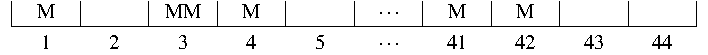
\includegraphics[width=.88\textwidth]{assets/chapter1/bins.pdf}\end{center}
可能的彩票数等于把六个标记放入44个格子的方法数.不过还可以进一步化简：只需记录标记与格子隔墙的排列.再注意，最外侧的两面墙不起作用.因此必须数清43面墙（44个格子产生45面墙，但忽略两端的墙）和六个标记的所有排列.一共有$43+6=49$个对象，可按$49!$种方式排列.然而，为除去重复排列，必须同时除以$6!$和$43!$，所以排列总数为
$$\frac{49!}{6!43!}=13,983,816.$$
\end{enumerate}
虽然上述推导都是通过一个例子完成的，但不难看出它们在一般情形下也成立.为求完整，表\ref{tab:1.2.1}汇总了这些情况.
\begin{table}[htbp]\centering
\caption{从$n$个对象中取$r$个的各种可能排列数}\label{tab:1.2.1}\index{SI0218@计数公式}
\renewcommand{\arraystretch}{1.8}
\begin{tabular}{ccc}\hline
 & 无放回 & 有放回\\
有序 & $\displaystyle\frac{n!}{(n-r)!}$ & $n^r$\\
无序 & $\displaystyle\binom nr$ & $\displaystyle\binom{n+r-1}{r}$\\\hline
\end{tabular}
\end{table}

\subsubsection{枚举结果}\label{sec:1.2.4}
当样本空间$S$是有限集，并且$S$中的所有结果等可能时，上一小节的计数技巧很有用.此时，只需数清事件中的结果数，就可以计算事件概率.为说明这一点，设$S=\{s_1,\ldots,s_N\}$是有限样本空间.所有结果等可能意味着对每个结果$s_i$都有$P(\{s_i\})=1/N$.由概率函数定义中的公理3，对任意事件$A$，有
$$P(A)=\sum_{s_i\in A}P(\{s_i\})=\sum_{s_i\in A}\frac1N=\frac{A\text{ 中的元素个数}}{S\text{ 中的元素个数}}.$$
对大型样本空间，可以使用计数技巧分别计算该式的分子和分母.
\begin{example}[扑克]\label{ex:1.2.18}
考虑从一副52张的标准扑克牌中选取一手五张牌.显然，这是无放回抽样.但为了明确可能结果（可能的牌型），必须决定把发牌看作逐张发出（有序）还是一次发出（无序）.如果要计算的事件依赖次序，例如前两张牌中出现一张A的概率，就必须使用有序结果.若事件不依赖次序，则可以使用无序结果.本例使用无序结果，因此样本空间由从52张牌中选出的所有五张牌组合构成.可能的牌组有$\binom{52}{5}=2,598,960$种.如果洗牌充分且随机发牌，则赋予每种可能牌组概率$1/2,598,960$是合理的.

现在通过计数事件中的结果来计算一些概率.拿到四张A的概率是多少？含四张A的牌组有多少种？四张牌已指定为A后，第五张牌有48种选择.因此，
$$P(\text{四张A})=\frac{48}{2,598,960},$$
概率小于五万分之一.使用定理\ref{thm:1.2.14}，只需稍微复杂一点的计数，就能计算拿到四张同点数牌的概率.四张同点数牌的点数有13种选择；确定这四张牌后，第五张牌有48种选择.因此，含四张同点数牌的牌组总数为$(13)(48)$，并且
$$P(\text{四张同点数牌})=\frac{(13)(48)}{2,598,960}=\frac{624}{2,598,960}.$$
要计算恰好一对的概率（不是两对，也不是三张同点数等），需要组合使用几种计数技巧.恰好一对的牌组数为
\begin{equation}\label{eq:1.2.11}
13\binom42\binom{12}{3}4^3=1,098,240.
\end{equation}
式\eqref{eq:1.2.11}来自定理\ref{thm:1.2.14}，因为
$$\begin{aligned}
13&=\text{指定一对的点数的方法数},\\
\binom42&=\text{从该点数中指定两张牌的方法数},\\
\binom{12}{3}&=\text{指定其余三个点数的方法数},\\
4^3&=\text{从这些点数中指定其余三张牌的方法数}.
\end{aligned}$$
因此，
$$P(\text{恰好一对})=\frac{1,098,240}{2,598,960}.$$
\end{example}
在例\ref{ex:1.2.18}这样的无放回抽样中，如果要计算不依赖次序的事件概率，则有序和无序样本空间都可以使用.无序样本空间中的每个结果对应有序样本空间中的$r!$个结果.因此，在有序样本空间中计数时，分子、分母各有一个$r!$因子，相消后得到的概率与在无序样本空间中计数相同.

有放回抽样则不同.无序样本空间中的每个结果对应有序样本空间中的一些结果，但所对应的个数各不相同.

\sourcepageanchor{45}

\begin{example}[有放回抽样]\label{ex:1.2.19}
考虑从$n=3$个对象中有放回地抽取$r=2$个对象.有序和无序样本空间中的结果如下：
\begin{center}\small
\begin{tabular}{ccccccc}\hline
无序 & $\{1,1\}$ & $\{2,2\}$ & $\{3,3\}$ & $\{1,2\}$ & $\{1,3\}$ & $\{2,3\}$\\
有序 & $(1,1)$ & $(2,2)$ & $(3,3)$ & $(1,2),(2,1)$ & $(1,3),(3,1)$ & $(2,3),(3,2)$\\
概率 & $1/9$ & $1/9$ & $1/9$ & $2/9$ & $2/9$ & $2/9$\\\hline
\end{tabular}
\end{center}
这些概率是把有序样本空间中的九个结果视为等可能而得到的.这对应于“有放回抽样”的通常解释：三个对象各以$1/3$的概率被选中；记录该对象后将其放回；混匀后再次从三个对象中选择一个，每个仍以$1/3$的概率被选中.可以看出，在这种抽样方式下，无序样本空间中的六个结果并非等可能.无序样本空间的结果数公式可用于枚举结果，但为了正确计算概率，必须对有序结果计数.
\end{example}
有些作者认为，在“把$r$个不可区分的球随机分配到$n$个可区分的罐子中”时，应给无序结果赋予相等概率.也就是说，随机选一个罐子并放入一球，重复$r$次.不记录放球的顺序，因此最终的结果$\{1,3\}$表示1号罐和3号罐各有一球.

但这种解释存在问题.假设两个人观察同一过程，观察者1记录放球顺序，观察者2不记录.观察者1会给事件$\{1,3\}$赋予概率$2/9$.观察者2看到的是完全相同的过程，也应给这个事件赋予概率$2/9$.然而，若把六个无序结果写在相同的纸片上，随机抽一片来决定球的放置方式，那么每个无序结果的概率就是$1/6$.于是观察者2会给事件$\{1,3\}$赋予概率$1/6$.

混淆的原因在于，“有放回”通常按上述依次抽样的方式理解，因此给事件$\{1,3\}$赋予概率$2/9$.这是正确的处理方式，因为概率应由抽样机制决定，而不是由球可区分还是不可区分来决定.

\sourcepageanchor{46}

\begin{example}[计算平均数]\label{ex:1.2.20}
为说明可区分／不可区分的处理方法，假设要计算从四个数
$$2,4,9,12$$
中有放回抽取四个数所得的所有可能平均数.例如，可能抽得$\{2,4,4,9\}$，平均数为4.75；也可能抽得$\{4,4,9,9\}$，平均数为6.5.如果只关心所抽数值的平均数，次序便不重要，因此不同样本总数可按无序、有放回抽样的方式计数.

不同样本总数为$\binom{n+n-1}{n}$.不过，要计算样本平均数的概率分布，必须数清某个平均数可以出现的不同方式.只有样本包含一个2、两个4和一个9时，才会出现4.75这个值.具有这种构成的可能样本如下表所示.
\begin{center}
\begin{tabular}{cl}
无序 & 有序\\\hline
$\{2,4,4,9\}$ & $(2,4,4,9),(2,4,9,4),(2,9,4,4),(4,2,4,9),$\\
 & $(4,2,9,4),(4,4,2,9),(4,4,9,2),(4,9,2,4),$\\
 & $(4,9,4,2),(9,2,4,4),(9,4,2,4),(9,4,4,2)$
\end{tabular}
\end{center}
有序样本总数为$n^n=4^4=256$，因此抽得无序样本$\{2,4,4,9\}$的概率为$12/256$.与此相比，如果认为无序样本等可能，就会给$\{2,4,4,9\}$及每个其他无序样本赋予概率$1/\binom{n+n-1}{n}=1/\binom74=1/35$.

为计算会产生$\{2,4,4,9\}$的有序样本数，可作如下论证.需要枚举四个数$\{2,4,4,9\}$的所有可能顺序，因此本质上属于第\ref{sec:1.2.3}节的计数方法1.样本可按$4\times3\times2\times1=24$种方式排序.但这里有重复计数，因为两个4的不同排列无法区分.例如，24种方式会把$\{9,4,2,4\}$数两次（若两个4不同，这样计数就没有问题）.为纠正这一点，除以$2!$（两个4有$2!$种排列），得到$24/2=12$个有序样本.一般说来，若有$k$个位置，$m$个不同的数分别重复$k_1,k_2,\ldots,k_m$次，则有序样本数为
$$\frac{k!}{k_1!k_2!\cdots k_m!}.$$
这种计数与\emph{多项分布}（multinomial distribution）有关，我们将在\hyperref[sec:4.6]{第4.6节}中讨论.图\ref{fig:1.2.2}是样本平均数概率分布的直方图，反映了对样本所作的多项式计数.\footnote{译注：原图注明写总体$\{2,4,4,9\}$，正文及直方图对应的却是$\{2,4,9,12\}$；下方保留原图注.}

\sourcepageanchor{47}

\begin{figure}[htbp]\centering
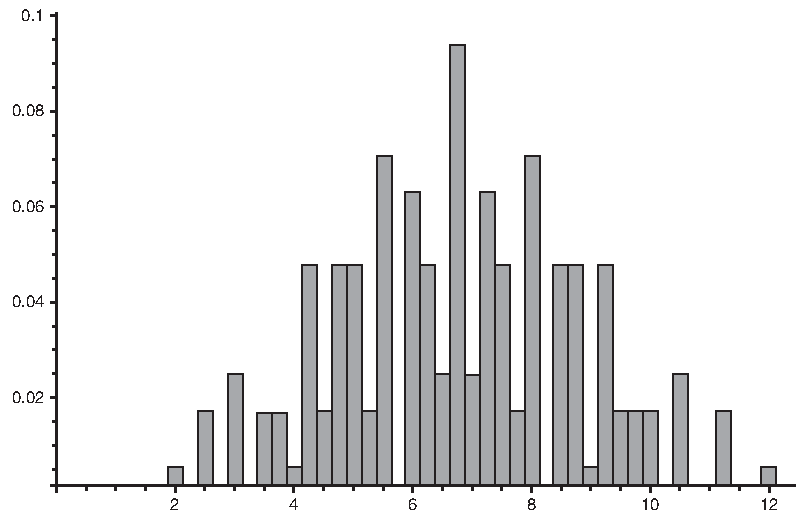
\includegraphics[width=.88\textwidth]{assets/chapter1/fig1-2-2.pdf}
\caption{从四个数$\{2,4,4,9\}$中有放回抽样所得平均数的直方图}\label{fig:1.2.2}
\end{figure}

图\ref{fig:1.2.2}还反映了一个需要进一步细化之处：两个不同的无序样本可能具有相同的平均数.例如，无序样本$\{4,4,12,12\}$和$\{2,9,9,12\}$的平均数都是8.第一个样本的概率为$3/128$，第二个样本的概率为$3/64$，因此取值8的概率为$9/128=.07$.\footnote{译注：原文使用等号；精确值为$0.0703125$，$.07$只是近似值.}关于如何构造这样的直方图，见\hyperref[ex:12.6.1]{例12.6.1}.本例中的计算是一种非常重要的统计技术——\emph{自助法}（bootstrap，\hyperref[bib:source114]{Efron与Tibshirani，1993}）的初级形式.我们将在\hyperref[sec:10.1.4]{第10.1.4节}再次讨论自助法.
\end{example}

% 用户授权疑误脚注：2026-11-04
